\documentclass[xetex,mathserif,serif]{beamer}

\usepackage{xunicode}
\usepackage{xltxtra}
\usepackage{color}
\usepackage{url}
\usepackage{listings}
\usepackage{fontspec}
\usepackage{geometry}
\usepackage{lastpage}
\usepackage{fancyhdr}
\usepackage{amsmath}
\usepackage{amsthm}
\usepackage{amssymb}
\usepackage{blkarray}
\usepackage{multicol}
\usepackage{relsize}

\definecolor{solarized@base03}{HTML}{002B36}
\definecolor{solarized@base02}{HTML}{073642}
\definecolor{solarized@base01}{HTML}{586e75}
\definecolor{solarized@base00}{HTML}{657b83}
\definecolor{solarized@base0}{HTML}{839496}
\definecolor{solarized@base1}{HTML}{93a1a1}
\definecolor{solarized@base2}{HTML}{EEE8D5}
\definecolor{solarized@base3}{HTML}{FDF6E3}
\definecolor{solarized@yellow}{HTML}{B58900}
\definecolor{solarized@orange}{HTML}{CB4B16}
\definecolor{solarized@red}{HTML}{DC322F}
\definecolor{solarized@magenta}{HTML}{D33682}
\definecolor{solarized@violet}{HTML}{6C71C4}
\definecolor{solarized@blue}{HTML}{268BD2}
\definecolor{solarized@cyan}{HTML}{2AA198}
\definecolor{solarized@green}{HTML}{859900}
\definecolor{yaleblue}{HTML}{0E4C92}

\setbeamertemplate{navigation symbols}{}
% \setbeamerfont{title}{family=\old}
% \setbeamerfont{author}{family=\tfont}%
% \setbeamerfont{frametitle}{family=\oldA}
% \setbeamerfont{date}{family=\dfont}

\setbeamertemplate{itemize items}{--}
\setbeamercolor*{item}{fg=black}

\defaultfontfeatures{Mapping=tex-text}
\hypersetup{pdfstartview={FitH}}

\newcommand{\old}[1]{\fontspec[Alternate=1,Ligatures={Common}]{Hoefler Text}\fontsize{18pt}{30pt}\selectfont #1}%
\newcommand{\oldA}[1]{\fontspec[Alternate=1,Ligatures={Common, Rare}]{Hoefler Text}\fontsize{12pt}{15pt}\selectfont #1}%
\newcommand{\oldB}[1]{\fontspec[Ligatures={Common}]{Didot}\fontsize{12pt}{15pt}\color{solarized@base02}\selectfont #1}%
\newcommand{\tfont}[1]{\fontspec[Alternate=1,Ligatures={Common}]{Hoefler Text}\fontsize{12pt}{20pt}\selectfont #1}%
\newcommand{\dfont}[1]{\fontspec[Ligatures={Common}]{Didot}\fontsize{12pt}{12pt}\selectfont #1}%

\newcommand{\minimize}{\mathop{\mathrm{minimize}}}
\newcommand{\argmin}{\mathop{\mathrm{arg\,min}}}
\newcommand{\argmax}{\mathop{\mathrm{arg\,max}}}
\newcommand{\st}{\mathop{\mathrm{subject\,\,to}}}

\newcommand\independent{\protect\mathpalette{\protect\independenT}{\perp}}
\def\independenT#1#2{\mathrel{\rlap{$#1#2$}\mkern2mu{#1#2}}}

\setlength{\parindent}{0pt}
\setlength{\parskip}{12pt}

\setromanfont [Ligatures={Common}, Numbers={OldStyle}, Variant=01,
 BoldFont={LinLibertine_RB.otf},
 ItalicFont={LinLibertine_RI.otf},
 BoldItalicFont={LinLibertine_RBI.otf}
 ]{LinLibertine_R.otf}



\begin{document}

%%%%%%%%%%%%%%%%%%%%%%%%%%%%%%%%%%%%%%%%%%%%%%%%%%%
\begin{frame}[fragile] \frametitle{}

\vfill

{\fontsize{0.7cm}{0cm}\selectfont Lecture 13 \\\vspace{0.2cm}
Solving Least Squares}\\\vspace{0.5cm}
28 October 2015

\vspace{2cm}

\begin{minipage}{0.6\textwidth}
Taylor B. Arnold \\
Yale Statistics \\
STAT 312/612
\end{minipage}
\hfill
\begin{minipage}{0.3\textwidth}\raggedleft

\includegraphics[scale=0.3]{../yale-logo.png}
\end{minipage}%

\end{frame}

%%%%%%%%%%%%%%%%%%%%%%%%%%%%%%%%%%%%%%%%%%%%%%%%%%%
\begin{frame}[fragile] \frametitle{}

{\color{yaleblue}\fontsize{16pt}{20pt}\selectfont Notes}

\begin{itemize}
\item Problem Set \#4 - Due today
\end{itemize}

\end{frame}

%%%%%%%%%%%%%%%%%%%%%%%%%%%%%%%%%%%%%%%%%%%%%%%%%%%
\begin{frame}[fragile] \frametitle{}

{\color{yaleblue}\fontsize{16pt}{20pt}\selectfont Goals for today}

\begin{itemize}
\item How to solve ordinary least squares (the right way!)
\item
\end{itemize}

\end{frame}

%%%%%%%%%%%%%%%%%%%%%%%%%%%%%%%%%%%%%%%%%%%%%%%%%%%
\begin{frame}[fragile] \frametitle{}

\begin{flushright}
{\color{yaleblue}\sc\fontsize{1cm}{0cm}\selectfont Solving least squares}
\end{flushright}

\end{frame}

%%%%%%%%%%%%%%%%%%%%%%%%%%%%%%%%%%%%%%%%%%%%%%%%%%%
\begin{frame}[fragile] \frametitle{}

When started looking at multivariate regression, I wrote down the
normal equations:
\begin{align*}
(X^t X) \widehat{\beta} &= X^t y
\end{align*}
Recall that these are called equations (plural) because we can think
of this as a set of $p$ simultaneous equations.

\end{frame}

%%%%%%%%%%%%%%%%%%%%%%%%%%%%%%%%%%%%%%%%%%%%%%%%%%%
\begin{frame}[fragile] \frametitle{}

For the last month we have been assuming that we solve this by
just taking the matrix inverse of $X^tX$ to yield the following:
\begin{align*}
 \widehat{\beta} &= (X^t X)^{-1} X^t y
\end{align*}

\end{frame}

%%%%%%%%%%%%%%%%%%%%%%%%%%%%%%%%%%%%%%%%%%%%%%%%%%%
\begin{frame}[fragile] \frametitle{}

For the last month we have been assuming that we solve this by
just taking the matrix inverse of $X^tX$ to yield the following:
\begin{align*}
 \widehat{\beta} &= (X^t X)^{-1} X^t y
\end{align*}

\end{frame}


%%%%%%%%%%%%%%%%%%%%%%%%%%%%%%%%%%%%%%%%%%%%%%%%%%%
\begin{frame}[fragile] \frametitle{}

Why might this be a problem? Well, consider the simple case where
we have $n = p = 2$ with the following:
\begin{align*}
X &= \left( \begin{array}{cc} 10^9 & -1 \\ -1 & 10^{-5} \end{array}\right) \\
\beta &= \left( \begin{array}{c} 1 \\ 1 \end{array}\right)
\end{align*}
\pause For simplicity, we'll even assume that there is no noise vector. Then
we have:
\begin{align*}
y &= \left( \begin{array}{cc} 10^9 & -1 \\ -1 & 10^{-5} \end{array}\right) * \left( \begin{array}{c} 1 \\ 1 \end{array}\right) \\
&= \left( \begin{array}{c} 10^9 - 1 \\ -0.99999 \end{array}\right)
\end{align*}

\end{frame}

%%%%%%%%%%%%%%%%%%%%%%%%%%%%%%%%%%%%%%%%%%%%%%%%%%%
\begin{frame}[fragile] \frametitle{}

Let's try running this in R:
\begin{verbatim}
> X  <- matrix(c(10^9, -1, -1, 10^(-5)), 2, 2)
> X
       [,1]   [,2]
[1,]  1e+09 -1e+00
[2,] -1e+00  1e-05
> beta <- c(1,1)
> y <- X %*% beta
> y
            [,1]
[1,]  1.0000e+09
[2,] -9.9999e-01
\end{verbatim}

\end{frame}

%%%%%%%%%%%%%%%%%%%%%%%%%%%%%%%%%%%%%%%%%%%%%%%%%%%
\begin{frame}[fragile] \frametitle{}

So far, so good. Now, because we have a square design matrix we
can invert it directly and solve $\beta = X^{-1} y$. This is not
a problem here:
\pause
\begin{verbatim}
> Xinv <- solve(X)
> Xinv %*% y
     [,1]
[1,]    1
[2,]    1
\end{verbatim}
\pause The correct $\beta$ is returned.

\end{frame}

%%%%%%%%%%%%%%%%%%%%%%%%%%%%%%%%%%%%%%%%%%%%%%%%%%%
\begin{frame}[fragile] \frametitle{}

However, what if we try to calculate this with the normal
equations? Here we need to invert the matrix $X^t X$.
\pause
\begin{verbatim}
> XtXinv <- solve(t(X) %*% X)
Error in solve.default(t(X) %*% X) :
  system is computationally singular: reciprocal
  condition number = 8.09999e-23
\end{verbatim}
\pause R knows that this is not going to be good, and refuses to
calculate the inverse by default.

\end{frame}

%%%%%%%%%%%%%%%%%%%%%%%%%%%%%%%%%%%%%%%%%%%%%%%%%%%
\begin{frame}[fragile] \frametitle{}

Suppose that we turn off this warning (by setting the tolerance
to zero); what happens?
\pause
\begin{verbatim}
> XtX <- t(X) %*% X
> Xty <- t(X) %*% y
> XtXinv <- solve(XtX, tol=0)
> XtXinv
           [,1]       [,2]
[1,] 1.0002e-08 1.0002e+01
[2,] 1.0002e+01 1.0002e+10
> betaHat <- XtXinv %*% Xty
> betaHat
             [,1]
[1,]    0.9999995
[2,] 1080.4998042
\end{verbatim}
\pause So, here we see the results of the numerical instability.
The returned $\widehat{\beta}$ is not equal to the correct $\beta$!

\end{frame}

%%%%%%%%%%%%%%%%%%%%%%%%%%%%%%%%%%%%%%%%%%%%%%%%%%%
\begin{frame}[fragile] \frametitle{}

So, other than inverting the matrix what are our options?

\pause We'll start by looking at three approachs, each of which
involves a matrix decomposition.

\end{frame}

%%%%%%%%%%%%%%%%%%%%%%%%%%%%%%%%%%%%%%%%%%%%%%%%%%%
\begin{frame}[fragile] \frametitle{}

Consider the qr-decomposition of the matrix $X^t X$:
\begin{align*}
X^t X &= Q R
\end{align*}
Where $Q$ is a square orthonormal matrix ($QQ^t = \mathbb{I}_p$)
and $R$ is an upper triangular matrix.

\end{frame}

%%%%%%%%%%%%%%%%%%%%%%%%%%%%%%%%%%%%%%%%%%%%%%%%%%%
\begin{frame}[fragile] \frametitle{}

Because $Q$ is orthonormal, we can calculate its inverse in an
easy and stable way, yielding the following:
\begin{align*}
X^t X \widehat{\beta} &= X^t y \\
Q R \widehat{\beta} &= X^t y \\
R \widehat{\beta} &= Q^t X^t y \\
R \widehat{\beta} &= v \\
\end{align*}
Where $v$ is just a compact way of writing $Q^t X^t y$.

\end{frame}

%%%%%%%%%%%%%%%%%%%%%%%%%%%%%%%%%%%%%%%%%%%%%%%%%%%
\begin{frame}[fragile] \frametitle{}

To solve the equation:
\begin{align*}
R b &= v
\end{align*}
We use a technique called \textit{backsolving}.

\end{frame}

%%%%%%%%%%%%%%%%%%%%%%%%%%%%%%%%%%%%%%%%%%%%%%%%%%%
\begin{frame}[fragile] \frametitle{}

The best way to describe the backsolve algorithm is with a
simple example. Consider the 3 by 3 matrix case:
\begin{align*}
\left(
\begin{array}{ccc} R_{1,1} & R_{1,2} & R_{1,3} \\
                   0       & R_{2,2} & R_{2,3} \\
                   0       & 0       & R_{3,3} \\
\end{array} \right) \left(\begin{array}{c} b_1 \\ b_2 \\ b_3 \end{array} \right)
 &= \left(\begin{array}{c} v1 \\ v2 \\ v3 \end{array} \right)
\end{align*}
\pause What is an obvious place to start?

\pause Well, we can see right away that:
\begin{align*}
b_3 &= \frac{v_3}{R_{3,3}}
\end{align*}

\end{frame}

%%%%%%%%%%%%%%%%%%%%%%%%%%%%%%%%%%%%%%%%%%%%%%%%%%%
\begin{frame}[fragile] \frametitle{}

Now, if we know $b_3$ what can we do as a next step?
\begin{align*}
\left(
\begin{array}{ccc} R_{1,1} & R_{1,2} & R_{1,3} \\
                   0       & R_{2,2} & R_{2,3} \\
                   0       & 0       & R_{3,3} \\
\end{array} \right) \left(\begin{array}{c} b_1 \\ b_2 \\ b_3 \end{array} \right)
 &= \left(\begin{array}{c} v1 \\ v2 \\ v3 \end{array} \right)
\end{align*}
\pause Well, now we can calculate
\begin{align*}
b_2 &= \frac{v_2}{R_{2,2}} +  \frac{R_{2,3} \cdot b_3}{R_{2,2}}
\end{align*}

\end{frame}

%%%%%%%%%%%%%%%%%%%%%%%%%%%%%%%%%%%%%%%%%%%%%%%%%%%
\begin{frame}[fragile] \frametitle{}

So, now for the final line of
\begin{align*}
\left(
\begin{array}{ccc} R_{1,1} & R_{1,2} & R_{1,3} \\
                   0       & R_{2,2} & R_{2,3} \\
                   0       & 0       & R_{3,3} \\
\end{array} \right) \left(\begin{array}{c} b_1 \\ b_2 \\ b_3 \end{array} \right)
 &= \left(\begin{array}{c} v1 \\ v2 \\ v3 \end{array} \right)
\end{align*}
By calculating the same thing:
\begin{align*}
b_1 &= \frac{v_1}{R_{1,1}} + \frac{R_{1,2} \cdot b_2}{R_{1,1}} + \frac{R_{1,3} \cdot b_3}{R_{1,1}}
\end{align*}

\end{frame}

%%%%%%%%%%%%%%%%%%%%%%%%%%%%%%%%%%%%%%%%%%%%%%%%%%%
\begin{frame}[fragile] \frametitle{}

You can see that this algorithm generalizes to solving
any linear system $Ab = x$ with an upper diagonal matrix $A$.
In only requires basic arithmetic and therefore has minimal
numerical issues.

\pause Notice that we never actually produce the inverse
matrix itself. We only apply and algorithm which produces
the inverse at any given point.

\end{frame}

%%%%%%%%%%%%%%%%%%%%%%%%%%%%%%%%%%%%%%%%%%%%%%%%%%%
\begin{frame}[fragile] \frametitle{}

Now, back to our example:
\begin{align*}
X^t X \widehat{\beta} &= X^t y \\
Q R \widehat{\beta} &= X^t y \\
R \widehat{\beta} &= Q^t X^t y \\
R \widehat{\beta} &= v \\
\end{align*}
We can then complete the final line by backsolving.

\end{frame}


%%%%%%%%%%%%%%%%%%%%%%%%%%%%%%%%%%%%%%%%%%%%%%%%%%%
\begin{frame}[fragile] \frametitle{}

We can calculate the qr decomposition in R:
\begin{verbatim}
> QR <- qr(XtX)
> QR
$qr
       [,1]         [,2]
[1,] -1e+18 1.000000e+09
[2,] -1e-09 9.998002e-11

$rank
[1] 1

$qraux
[1] 2.000000e+00 9.998002e-11

$pivot
[1] 1 2
\end{verbatim}

\end{frame}

%%%%%%%%%%%%%%%%%%%%%%%%%%%%%%%%%%%%%%%%%%%%%%%%%%%
\begin{frame}[fragile] \frametitle{}

To get the actual matricies, we need to run two functions
to calcualte them from the R object:
\begin{verbatim}
> Q <- qr.Q(QR)
> R <- qr.R(QR)
\end{verbatim}
And then we can solve the normal equations:
\begin{verbatim}
> v <- t(Q) %*% Xty
> backsolve(R, v)
     [,1]
[1,]    1
[2,]    0
\end{verbatim}
\pause Okay, so still not the correct $\beta$ (which should
have both components equal to $1$), but still a lot better
than the completely unstable solution we had previously.

\end{frame}

%%%%%%%%%%%%%%%%%%%%%%%%%%%%%%%%%%%%%%%%%%%%%%%%%%%
\begin{frame}[fragile] \frametitle{}

Note that we can do this all in one step automatically inside
of R. However, by default we get a warning this this is a bad
idea:
\begin{verbatim}
> betaHat <- qr.solve(XtX, Xty)
Error in qr.solve(XtX, Xty) : singular matrix 'a' in solve
\end{verbatim}
\pause Turning this off yields the result that we calculated
ourselves:
\begin{verbatim}
> betaHat <- qr.solve(XtX, Xty, tol=0)
> betaHat
     [,1]
[1,]    1
[2,]    0
\end{verbatim}

\end{frame}

%%%%%%%%%%%%%%%%%%%%%%%%%%%%%%%%%%%%%%%%%%%%%%%%%%%
\begin{frame}[fragile] \frametitle{}

Another decompostion that is useful for solving this
problem is the Cholseky decomposition, which writes
a matrix as $U^t U$ for some upper diagonal matrix $U$.
If we use this the solution can be calculated by forward
solving (the same as backsolving, but for a lower diagonal
matrix) and then backsolving.

\end{frame}

%%%%%%%%%%%%%%%%%%%%%%%%%%%%%%%%%%%%%%%%%%%%%%%%%%%
\begin{frame}[fragile] \frametitle{}

In R, we can do this as follows:
\begin{verbatim}
> U <- chol(XtX)
> U
      [,1]          [,2]
[1,] 1e+09 -1.000000e+00
[2,] 0e+00  9.999001e-06
\end{verbatim}
And solving yields:
\begin{verbatim}
> betaHat <- backsolve(U, forwardsolve(t(U), Xty))
> betaHat
     [,1]
[1,]    1
[2,]    0
\end{verbatim}
\pause So this gives the same solution as the QR decomposition.

\end{frame}

%%%%%%%%%%%%%%%%%%%%%%%%%%%%%%%%%%%%%%%%%%%%%%%%%%%
\begin{frame}[fragile] \frametitle{}

A final technique is the eigenvalue decomposition, which
writes a matrix as $Q D Q^t$ for $Q$ orthogonal and
$D$ a diagonal matrix.

\pause To solve this we simply multiply by $Q^t$ on the left,
divide by the diagonal of $D$, and multiply by $Q$.

\end{frame}

%%%%%%%%%%%%%%%%%%%%%%%%%%%%%%%%%%%%%%%%%%%%%%%%%%%
\begin{frame}[fragile] \frametitle{}

In R, the eigen value decomposition is given by the function
\texttt{eigen}:
\begin{verbatim}
> EIGEN <- eigen(XtX)
> EIGEN
$values
[1] 1.000000e+18 9.998002e-11

$vectors
       [,1]   [,2]
[1,] -1e+00 -1e-09
[2,]  1e-09 -1e+00
\end{verbatim}

\end{frame}

%%%%%%%%%%%%%%%%%%%%%%%%%%%%%%%%%%%%%%%%%%%%%%%%%%%
\begin{frame}[fragile] \frametitle{}

And to solve the linear system we see that:
\begin{verbatim}
> Q <- EIGEN$vectors
> D <- diag(EIGEN$values)
> step01 <- t(Q) %*% Xty
> step02 <- step01 / diag(D)
> betaHat <- Q %*% step02
> betaHat
       [,1]
[1,]  1e+00
[2,] -1e-09
\end{verbatim}
Which is very close to what the other methods yielded.

\end{frame}

%%%%%%%%%%%%%%%%%%%%%%%%%%%%%%%%%%%%%%%%%%%%%%%%%%%
\begin{frame}[fragile] \frametitle{}

So we have three methods: the Cholesky decomposition which involves
two diagonal solves (one back and one forward), the QR which
involves one diagonal solve and one matrix multiplication,
and the eigenvalue decompositon which involves two matrix
multiplications.

\pause Each of these has its own uses and pros and cons. We
will likely discuss some of these over the next few weeks.
For now though, we are mostly concerned with the fact that
none of them return the correct $\widehat{\beta}$ that we
expect.

\end{frame}

%%%%%%%%%%%%%%%%%%%%%%%%%%%%%%%%%%%%%%%%%%%%%%%%%%%
\begin{frame}[fragile] \frametitle{}

So far we have only taken decompositions of square matricies.
The QR decomposition actually yields a solution even for rectangular
matricies. We can write the decomposition of the $n$-by-$p$
matrix A as:
\begin{align*}
A &= \left[ \begin{array}{cc} Q_1 & Q_2 \end{array} \right] \cdot
\left[ \begin{array}{c} R_1 \\ 0 \end{array} \right]
\end{align*}
With $R_1$ being a $p$-by-$p$ matrix, $Q_1$ a $n$-by-$p$ matrix
and $Q_2$ a $n$-by-$(n-p)$ matrix. This is sometimes known as
the \textit{thin} QR decomposition. Notice that $Q_2$ is not unique,
nor is it even needed to reconstruct $A$.

\end{frame}

%%%%%%%%%%%%%%%%%%%%%%%%%%%%%%%%%%%%%%%%%%%%%%%%%%%
\begin{frame}[fragile] \frametitle{}

Now, let's take a step back from the normal equations and consider
the sum of squares directly:
\begin{align*}
|| y - X \beta ||_2^2 &= (y - X \beta)^t (y - X\beta)
\end{align*}
\pause Notice that if we have an orthonormal matrix $Q$ we can insert this
into the middle of the sum of squares without changing the value:
\begin{align*}
|| Q (y - X \beta) ||_2^2 &= (y - X \beta)^t Q^t Q (y - X\beta) \\
&= (y - X \beta)^t Q^t Q (y - X\beta) \\
&= (y - X \beta)^t (y - X\beta) \\
&= || y - X \beta ||_2^2
\end{align*}

\end{frame}

%%%%%%%%%%%%%%%%%%%%%%%%%%%%%%%%%%%%%%%%%%%%%%%%%%%
\begin{frame}[fragile] \frametitle{}

On its own, this is an important (though hopefully unsurprising)
result. We can rotate the problem by any orthonormal matrix and
return the same sum of squares; this will be very useful in
several ways.

\end{frame}

%%%%%%%%%%%%%%%%%%%%%%%%%%%%%%%%%%%%%%%%%%%%%%%%%%%
\begin{frame}[fragile] \frametitle{}

On of those ways comes from taking the QR decomposition of the
matrix $X$ and rotating the space by the transpose of
the resulting $Q$.

\pause Then, we can then write the squared residuals as
\begin{align*}
Q^t (y - X \beta)&=
\left[ \begin{array}{c} Q_1^t \\ Q_2^t \end{array} \right] y -
\left[ \begin{array}{c} Q_1^t \\ Q_2^t \end{array} \right] \times
\left[ \begin{array}{cc} Q_1 & Q_2 \end{array} \right] \cdot
\left[ \begin{array}{c} R_1 \\ 0 \end{array} \right] \beta \\
&= \left[ \begin{array}{c} Q_1^t \\ Q_2^t \end{array} \right] y -
\left[ \begin{array}{c} R_1 \\ 0 \end{array} \right] \beta
\end{align*}
Notice that the final $n-p$ rows of the resulting vector do not
involve $\beta$ as they are canceled out by the $0$.

\end{frame}

%%%%%%%%%%%%%%%%%%%%%%%%%%%%%%%%%%%%%%%%%%%%%%%%%%%
\begin{frame}[fragile] \frametitle{}

So we now have the following equation:
\begin{align*}
||y - X \beta ||_2^2 &=||Q^t (y - X \beta) ||_2^2 \\
&= ||Q_1^t y - R_1 \beta||_2^2 +
||Q_2^t y ||_2^2
\end{align*}
\pause This is actually very useful, because we can
minimize over $\beta$ by just minimizing the first
term, which can actually be set exactly equal to zero:
\begin{align*}
Q_1^t y &= R_1 \beta \\
R_1^{-1} Q_1^t y &= \beta
\end{align*}
Though, as you now know, we would actually backsolve
rather than take the actual inverse of $R_1$.

\end{frame}

%%%%%%%%%%%%%%%%%%%%%%%%%%%%%%%%%%%%%%%%%%%%%%%%%%%
\begin{frame}[fragile] \frametitle{}

So now, let's try this on our problem:
\begin{verbatim}
> E <- qr(X)
> Q <- qr.Q(E)
> R <- qr.R(E)
> backsolve(R, t(Q) %*% y)
     [,1]
[1,]    1
[2,]    1
\end{verbatim}
\pause Thankfully, this yields the expected result!

\end{frame}

%%%%%%%%%%%%%%%%%%%%%%%%%%%%%%%%%%%%%%%%%%%%%%%%%%%
\begin{frame}[fragile] \frametitle{}

Carefully note though, that there is some numerical
error that is hidden by the default precision of R:
\begin{verbatim}
> options(digits=22)
> backsolve(R, t(Q) %*% y)
                         [,1]
[1,] 1.0000000000000000000000
[2,] 0.9999999999982769338658
\end{verbatim}

\end{frame}

%%%%%%%%%%%%%%%%%%%%%%%%%%%%%%%%%%%%%%%%%%%%%%%%%%%
\begin{frame}[fragile] \frametitle{}

Carefully note though, that there is some numerical
error that is hidden by the default precision of R:
\begin{verbatim}
> options(digits=22)
> backsolve(R, t(Q) %*% y)
                         [,1]
[1,] 1.0000000000000000000000
[2,] 0.9999999999982769338658
\end{verbatim}

\end{frame}


%%%%%%%%%%%%%%%%%%%%%%%%%%%%%%%%%%%%%%%%%%%%%%%%%%%
\begin{frame}[fragile] \frametitle{}

This method has a nice geometric interpretation in relationship
to the geometry of least squares:
\pause

\begin{center}
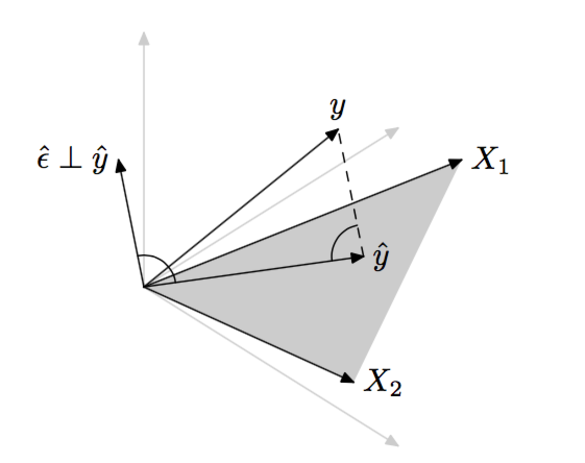
\includegraphics[width=4in]{img/olsGeom.pdf}
\end{center}

\end{frame}

%%%%%%%%%%%%%%%%%%%%%%%%%%%%%%%%%%%%%%%%%%%%%%%%%%%
\begin{frame}[fragile] \frametitle{}

What is really going on here?
\begin{verbatim}
> options(digits=22)
> betaHat <- qr.solve(XtX, Xty, tol=0)
                         [,1]
[1,] 0.9999999990000000282819
[2,] 0.0000000000000000000000
> XtX %*% betaHat - Xty
     [,1]
[1,]    0
[2,]    0
\end{verbatim}
\pause Directly solving the normal equations produces
solutions that correctly give $X^tX \beta = X^ty$.

\end{frame}

%%%%%%%%%%%%%%%%%%%%%%%%%%%%%%%%%%%%%%%%%%%%%%%%%%%
\begin{frame}[fragile] \frametitle{}

Now, let us try this on a non-square matrix to illustrate
what happens in a more typically setting.

\pause We construct a dataset with $25$ highly correlated
columns:
\begin{verbatim}
> options(digits=22)
> n <- 1000
> p <- 25
> alpha <- 1e-5
> X <- matrix(runif(n*p), ncol=p)
> X <- alpha * X + matrix(rnorm(n), nrow=n, ncol=p)
>
> beta <- runif(p)
> y <- X %*% beta + rnorm(n,sd=0.5)
> cor(X[,1], X[,2])
[1] 0.9999999999916668880218
\end{verbatim}

\end{frame}

%%%%%%%%%%%%%%%%%%%%%%%%%%%%%%%%%%%%%%%%%%%%%%%%%%%
\begin{frame}[fragile] \frametitle{}

Now let us try our two methods for solving the ordinary
least squares problem.
\end{frame}

%%%%%%%%%%%%%%%%%%%%%%%%%%%%%%%%%%%%%%%%%%%%%%%%%%%
\begin{frame}[fragile] \frametitle{}

{\bf Normal equations (Cholesky)}
\begin{verbatim}
> XtX <- t(X) %*% X
> Xty <- t(X) %*% y
>
> U <- chol(XtX)
> betaChol <- backsolve(U, forwardsolve(t(U),Xty))
\end{verbatim}

\end{frame}

%%%%%%%%%%%%%%%%%%%%%%%%%%%%%%%%%%%%%%%%%%%%%%%%%%%
\begin{frame}[fragile] \frametitle{}

{\bf QR-decomposition}

\begin{verbatim}
> QR <- qr(X)
> Q <- qr.Q(QR)
> R <- qr.R(QR)
> dim(Q)
[1] 1000   25
> dim(R)
[1] 25 25
>
> betaQR <- backsolve(R, t(Q) %*% y)
\end{verbatim}

\end{frame}

%%%%%%%%%%%%%%%%%%%%%%%%%%%%%%%%%%%%%%%%%%%%%%%%%%%
\begin{frame}[fragile] \frametitle{}

Look at the quantiles of the results
\begin{verbatim}
> options(digits=8)
> quantile(beta)
          0%          25%          50%          75%         100%
0.0042836969 0.2510972756 0.5518817164 0.8211262035 0.9827954113
> quantile(betaQR)
          0%          25%          50%          75%         100%
-15406.39499  -1497.12478    134.70958   3361.91288   7500.65667
> quantile(betaChol)
          0%          25%          50%          75%         100%
-15405.61168  -1499.20582    134.37818   3361.92816   7499.46646
\end{verbatim}
\pause The predicted values are significantly larger in magnitude
than the true beta values!

\end{frame}

%%%%%%%%%%%%%%%%%%%%%%%%%%%%%%%%%%%%%%%%%%%%%%%%%%%
\begin{frame}[fragile] \frametitle{}

Comparison of regression vectors:
\begin{verbatim}
> sqrt(sum(abs(betaQR - betaChol)^2)) / sqrt(sum(abs(betaQR)^2))
[1] 0.00047420293
\end{verbatim}
And the predicted values:
\begin{verbatim}
> sqrt(sum(abs(X %*% betaQR - X%*% betaChol)^2)) /
+  sqrt(sum(abs(X %*% betaQR)^2))
[1] 2.7345493e-06
\end{verbatim}

\pause
{\bf These represent numerical imprecision; the difference between
 the two methods of calculating the regression vector}

\end{frame}

%%%%%%%%%%%%%%%%%%%%%%%%%%%%%%%%%%%%%%%%%%%%%%%%%%%
\begin{frame}[fragile] \frametitle{}

Now, compare the predicted value (QR) to the actual $\beta$
and $y$ values:
\begin{verbatim}
> sqrt(sum(abs(betaQR - beta)^2)) /
+   sqrt(sum(abs(betaQR)^2))
[1] 0.99999031
\end{verbatim}
And the predicted values:
\begin{verbatim}
> sqrt(sum(abs(X %*% betaQR - X %*% beta)^2)) /
+  sqrt(sum(abs(X %*% betaQR)^2))
[1] 0.0055357352
\end{verbatim}

\pause
{\bf These represent the statistical error.} They are much worse,
particularly for the regression vector.

\end{frame}

%%%%%%%%%%%%%%%%%%%%%%%%%%%%%%%%%%%%%%%%%%%%%%%%%%%
\begin{frame}[fragile] \frametitle{}

Notice that the normal equations are solved very well,
even though the regression vector is not:
\begin{verbatim}
> max(abs(t(X) %*% X %*% betaQR - t(X) %*% y))
[1] 5.7070793e-08
> max(abs(t(X) %*% X %*% betaChol - t(X) %*% y))
[1] 9.7188604e-09
\end{verbatim}

\end{frame}

%%%%%%%%%%%%%%%%%%%%%%%%%%%%%%%%%%%%%%%%%%%%%%%%%%%
\begin{frame}[fragile] \frametitle{}

What is going on here? We have seen this before when we had a model
that was generated by the following:
\begin{align*}
Y = X_1 + X_2 + \text{noise}
\end{align*}
\pause If $X_1$ and $X_2$ are highly correlated it will be very difficult
to distinguish the true model from any of the following:
\begin{align*}
Y &= 2 \times X_1 + \text{noise} \\
Y &= 3 \times X_1 - X_2 + \text{noise} \\
Y &= 200 \times X_1 - 199 \times X_2 + \text{noise}
\end{align*}
Notice how the coefficents can easily be orders of magnitude larger
than the true model.

\end{frame}

%%%%%%%%%%%%%%%%%%%%%%%%%%%%%%%%%%%%%%%%%%%%%%%%%%%
\begin{frame}[fragile] \frametitle{}

{\bf The big picture}

Why do we (i.e., STAT 612) care about numerical precision?

\pause It is very difficult to construct non-trival
datasets that exhibit numerically unstable results (at least,
without doing something that makes no sense in practice). \pause
The main reason we are still interested is because methods for
addressing the statistical error mimic (and are motivated by)
the methods for fixing numerical errors.

\pause Bad statistical noise is {\bf very} common even with
only moderately correlated covariates!

\end{frame}

% %%%%%%%%%%%%%%%%%%%%%%%%%%%%%%%%%%%%%%%%%%%%%%%%%%%
% \begin{frame}[fragile] \frametitle{}

% The question is, given a system of linear
% equations:
% \begin{align*}
% A b = y
% \end{align*}
% What does the set of numerically allowable results look
% like?

% \end{frame}

% %%%%%%%%%%%%%%%%%%%%%%%%%%%%%%%%%%%%%%%%%%%%%%%%%%%
% \begin{frame}[fragile] \frametitle{}

% Let $\beta$ be the true solution, calculatable only by a machine
% with perfect precision. Then any other $b$ such that:
% \begin{align*}
% ||Ab - y|| \leq \epsilon
% \end{align*}
% Gives us:
% \begin{align*}
% ||Ab - A\beta|| \leq \epsilon
% \end{align*}

% \end{frame}

% %%%%%%%%%%%%%%%%%%%%%%%%%%%%%%%%%%%%%%%%%%%%%%%%%%%
% \begin{frame}[fragile] \frametitle{}

% So from a prediction standpoint, that is, calculating $Ab$, the
% difference between solutions is not a concern. Howerver, if we
% are interested in
% \begin{align*}
% ||Ab - A\beta|| \leq \epsilon
% \end{align*}

% \end{frame}

\end{document}











